\section{Theory}
When a current-carrying semiconductor or metal is kept in a magnetic field, the
charge carriers of the semiconductor experience a force in a direction
perpendicular to both the magnetic field and the current. At equilibrium, a voltage
appears at the semiconductor edges. Measurement of Hall effect is an important tool is determining mobilities of electrons and holes in semiconductors where simple measurements of conductivity is insufficient to distinguish the both. 
% To observe Hall effect, consider a crystal, with contacts 1, 2 and 3 perpendicular to the magnetic field $H$ in the $z$-direction. When a voltage $V_x$ is applied between contacts 1 and 2 to induce current flow through the crystal in $x$-direction, a voltage will arise across contacts 3 and 4 in the $y$-direction. Assuming all carriers possess equal drift velocity, it is easy to compute this (Hall) voltage. To do so, we make one of the two assumptions,
Let us consider two scenarios: (a) that there is only one kind of carrier present, and (b) that both types of carriers are present.

\subsection{One type of Carrier}

Consider a crystal, with contacts 1, 2 and 3 perpendicular to the magnetic field $H$ in the $z$-direction. When a voltage $V_x$ is applied between contacts 1 and 2 to induce current flow through the crystal in $x$-direction, a voltage will arise across contacts 3 and 4 in the $y$-direction (Fig. \ref{hall}). 

\begin{figure}
    \centering
    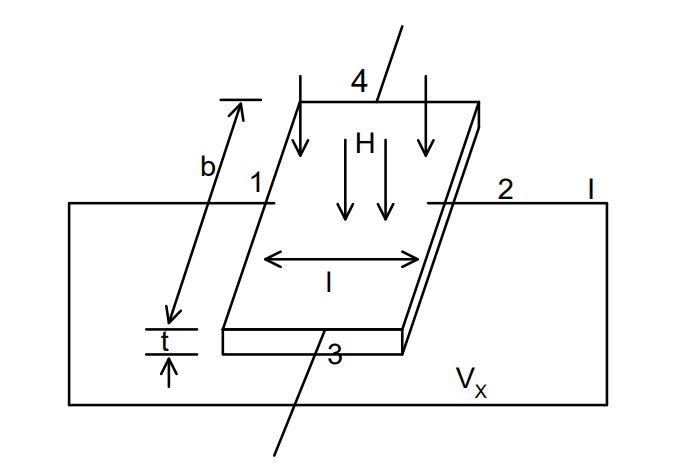
\includegraphics[width=0.7\columnwidth]{images/hall.png}
    \caption{Schematic arrangement for the measurement of the Hall Effect of a crystal}
    \label{hall}
\end{figure}

Under the Hall voltage, the magnetic force on the carriers is $\vv{F}_m=e\vv{E}_m=e(\vv{v}\times\vv{H})$ and is compensated by the force $\vv{F_h}$ due to the Hall fields $\vv{E_h}$. The electric field $\vv{E_m}$ is along the $y$-axis and is provided by $E_m = vH = \mu E_x H$, where the carrier mobility $\mu$ is determined by $v = \mu E_x$, and $E_x$ is the applied electric field along the $x$-axis. This is because $\vv{v}$ is along the $x$-axis, and $\vv{H}$ is along the $z$-axis. $\sigma E_x = J_x$ describes the relationship between the electric field, current density, and conductivity. The Hall coefficient $R_H$ is given by:

\begin{align}
    \label{eq:1}
    \abs{R_H}=\frac{E_m}{J_xH}=\frac{1}{ne}=\frac{V_y t}{I_xH}
\end{align}

here $t$ is the thickness of the sample. Thus, for a fixed magnetic field and input current, the Hall voltage is proportional to $1/n$.

\subsection{Two Types of Carriers}
We observe that the Hall voltage for p-type carriers (holes) has the opposite sign from that for n-type carriers (electrons) for the same electric field $E_x$. Consequently, the sign of the Hall coefficient $R_H$ is also different for the two types of carriers. Both types of carriers experience a transverse motion due to the Hall field $E_y$, which fails to counteract the magnetic force acting on them. However, since no current flows through contacts 3, 4, and 5, the net transverse transfer of charge remains zero.

In the x-direction, we have:

\begin{align}
    e(v^+_xp-v^-_xn)=J_x,
    \label{eq:x_direction}
\end{align}

where $v^+_x$ has the opposite sign from $v^-_x$. The carrier mobility $\mu$ is always a positive number, and the total current density $\sigma$ is given by:

\begin{align}
    e(\mu^+p+\mu^-n)=\sigma.
    \label{eq:total_current_density}
\end{align}

The velocity of carriers in the y-direction is defined as:

\begin{align}
    v^-_y=\frac{F\tau}{2m^*},
    \label{eq:y_direction}
\end{align}

where $m^*$ is the effective mass of carriers, and $\tau$ is the mean time between collisions. The Hall coefficient is given by:

\begin{align}
    R_H=\frac{E_H}{J_xH}=\frac{E_H}{\sigma E_xH}=\frac{(\mu^2_hp-\mu^2_en)}{e(\mu_hp+\mu_en)^2},
    \label{eq:hall_coefficient}
\end{align}

where $E_H$ is the Hall electric field, and $H$ is the magnetic field strength.

Since the mobilities $\mu_h$ and $\mu_e$ are functions of temperature, the Hall coefficient is also a function of temperature and may become zero and even change sign. In general, $\mu_e > \mu_h$, so Hall coefficient inversion can only occur if $p > n$. Therefore, Hall coefficient inversion is characteristic of only p-type semiconductors. At the point of zero Hall coefficient, it is possible to determine the ratio of mobilities.

The carrier concentration $n$ can be calculated from the hall coefficient using,

\begin{align} \label{eq:6}
    R_H = \frac{1}{ne}
\end{align}

Mobility $\mu$ is a measure of how quickly charge
carriers respond to an electric field and is calculated
using,

\begin{align} \label{eq:7}
    \mu = \frac{\sigma}{ne}
\end{align}

% =================================================
\section{Experimental Setup}
Fig. \ref{expt} shows the experimental setup for observing Hall effect. A detailed list of all the apparatus required is listed below.

\subsection*{Apparatus}

\begin{enumerate}
    \item Hall probe (Ge: p \& n types, Si: n-type)
    \item Oven
    \item Temperature sensor
    \item Hall Effect Set-up (DHE-22)
    \item Electromagnet (EMU-50V)
    \item Constant Current Power Supply (DPS-50)
    \item Digital Gaussmeter (DGM-102)
\end{enumerate}


\begin{figure}
    \centering
    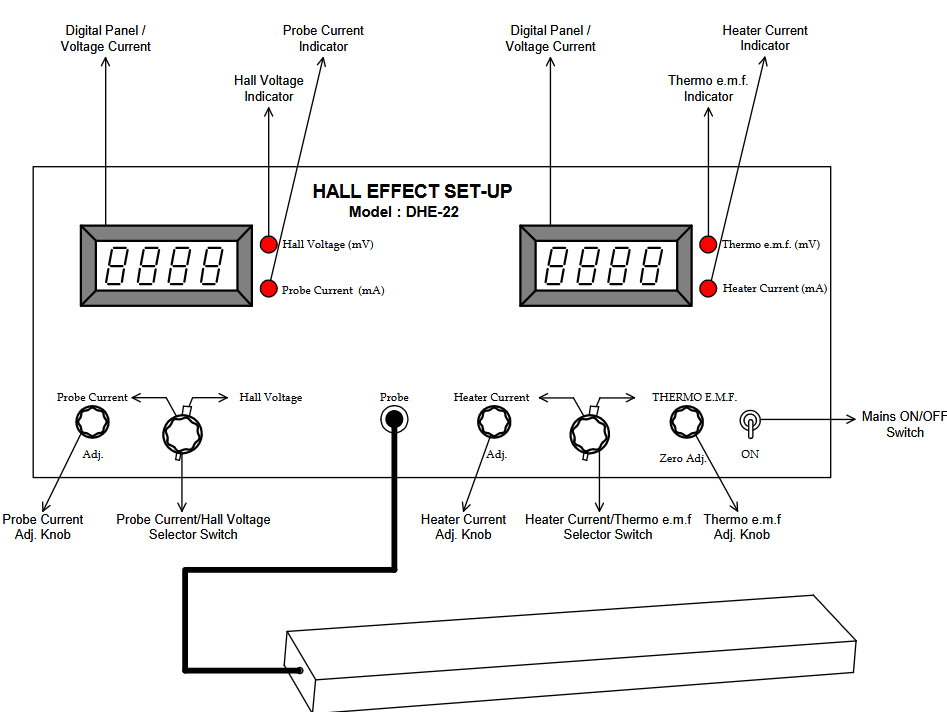
\includegraphics[width=1\columnwidth]{images/expt.png}
    \caption{Panel Diagram of the Hall effect set up}
    \label{expt}
\end{figure}